\chapter{Project Expectations}
\textbf{Showman and SEMI Sound - Background} \\
SEMI Sound is a startup founded by \textbf{Se}bastian Wolff and \textbf{Mi}nik Nathanielsen Olsen to develop and produce technologies for touring artists. Both Sebastian and Minik have many years of touring experience  as musician and sound engineer respectively. The concept for Showman was born around 2013-2014 after a series of performances with Sebastian's band (who employs Minik as backliner and monitor audio engineer), when the performances suffered technical difficulties caused by a malfunctioning hard disk recorder used for playback of backing tracks. \newline

Preparation for a tour is commonly referred to as \textit{pre-production}. During pre-production for a Summer tour in 2018, the band abandoned the idea of re-using the hard disk recorder in favor of the LP-16 Live Player as a temporary solution; Showman's additional features are needed for the next tour cycle. This motivated Minik to develop the Showman concept further and use the band as betatesters. Inspired by this, Minik decided to develop Showman as NSI Startup Factory as part of his apprenticeship period before continuing the project as part of the Bachelor's Project. To avoid a 6-month gap, Minik swapped 5th and 6th semester in order to work full-time on the project without interruptions. \newline

\subsection{Workplace}
\textbf{Workplace} \\
After initial project proposal was accepted, an application for project working space was filed to secure an assigned working space at the university campus. As of this document's handin, no working space has been assigned yet as deadline for application handin is January 11th. \\

Meeting with supervisor before initiating work on this document, it was announced that the project will be supervised jointly with 2 other projects who also work independently. Supervisor proposes that the 3 project share workplace to encourage a better work ethic which can be elusive on solo projects. \\

\textbf{Lab work} \\
Additionally, access to ASE's lab is crucial for the project when implementing and testing design. \\

\textbf{Working from home} \\
Living in Esbjerg, some 180 kilometers from ASE, it is expected to do some work at home as well. However, primary workplace during the weekdays is at ASE. \\

\subsection{Platform}
Initially, the \textbf{HDMI Audio EI3 EZ-Extender} (https://www.analog.com/en/design-center/evaluation-hardware-and-software/evaluation-boards-kits/eI3-hdmiaudio.html\#eb-overview) evaluation board was chosen as platform for Showman prototype. But it is not available at the moment, but \textit{used} boards are available online. \\

\begin{figure}[H]
\centering
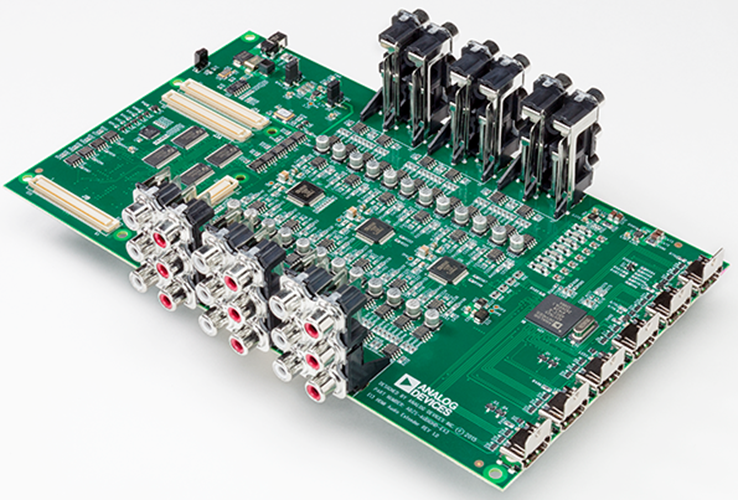
\includegraphics[scale=1]{./pictures/ei3.png}
\caption{Initial platform for development: \textbf{HDMI Audio EI3 EZ-Extender}. Rejected as it is currently unavailable from the vendor.}
\label{fig:ei3.png}
\end{figure}

For the audio part of Showman, \textbf{EVAL-21469-EZLITE} (https://www.analog.com/en/design-center/evaluation-hardware-and-software/evaluation-boards-kits/21469-ezlite.html\#eb-overview) is now the chosen platform. \\

\begin{figure}[H]
\centering
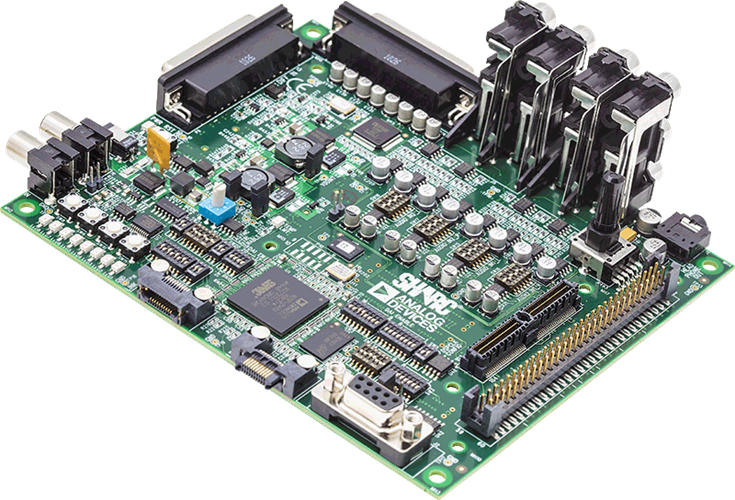
\includegraphics[scale=0.4]{./pictures/ADZS.png}
\caption{Requested platform for development: \textbf{EVAL-21469-EZLITE}.}
\label{fig:ADZS.png}
\end{figure}

\textbf{Price:} 574.20 USD + shipping \\ 

Research on video part is ongoing at the moment.

\subsection{Project Funding}
\subsubsection{Foundations}
As the price for the ADSP-2146x EZ-KIT Lite exceeds the maximum for university expense coverage, project funding from the university is not available. The necessary project funding need to be covered by external funds from initiatives such as InnoFounder, InnoBooster, etc. Applications for funding is currently in the works and essential material needed before the project begins is currently covered by Minik. \\

\subsubsection{Grants}
Concurrently with funding applications, applications for grants and donations are also in the works. \\

\subsubsection{Private Funding}
If applications from foundations and grants are refused, necessary funding will be covered by private funds from own savings. \\

\subsection{Beta Testers}
Having a large network of musicians, sound engineers and other touring personnel, a 2 other bands have been recruited as betatesters when the project is ready to test Showman. \newline
